\documentclass[fleqn,11pt]{SelfArx} 
%\setlength{\fboxrule}{0.75pt} % Width of the border around the abstract
\definecolor{color1}{RGB}{0,0,100} % Color of the article title and sections
\definecolor{color2}{RGB}{0,0,0} % Color of the boxes behind the abstract and headings
\usepackage{hyperref} % Required for hyperlinks
\hypersetup{hidelinks,colorlinks,breaklinks=true,urlcolor=color2,citecolor=color1,linkcolor=color1,bookmarksopen=false,pdftitle={Title},pdfauthor={Author}}

%----------------------------------------------------------------------------------------
%	ARTICLE INFORMATION
%----------------------------------------------------------------------------------------
\PaperTitle{Nuclear receptor variation in mice} % Article title

\Authors{Beratis, Alexander, Iacob, Diana, Boyanova, Dr. Desislava\textsuperscript{1}, Mewes, Prof. Dr. Hans-Werner\textsuperscript{1}} % Authors
\affiliation{\textsuperscript{1}\textit{Institute of Bioinformatics and Systems Biology, Helmholtz Zentrum M�nchen, German Research Center for Environmental Health,}} % Author affiliation

\Keywords{Nuclear receptors --- SNPs --- Gene variation} % Keywords
\newcommand{\keywordname}{Keywords} % Defines the keywords heading name

%----------------------------------------------------------------------------------------
%	ABSTRACT
%----------------------------------------------------------------------------------------

\Abstract{\textit{Nuclear receptors (NRs) are important signaling mediators in cells due to their ability to act as receptors and transcription factors. These molecules are activated by ligands and regulate critical functions in cell control, inflammation, fibrosis and tumor formation. Nuclear receptors act on the metabolism and signaling of cells by changing the expression of target genes. Here, we will investigate the knockout phenotypes and genetic variation of mouse NRs. We will first create an assembly of all known mouse SNPs in the vicinity of mouse NR genes (+-1Mbp up-or downstream). In a second step, phenotype information for genetic knockouts and genetic variation data will be included. Knockout phenotypes are available from the MGI database, while the Mouse Phenome Database provides SNPs from various mouse strains, which can be correlated to extreme phenotypes, measured in these mouse strains. The goal of this analysis is to find NR SNPs in mice that influence changes in biological parameters such as body weight, body fat and other phenotypic traits. Furthermore, we will couple these findings to phenotypes observed in mice with a targeted or spontaneous mutation of the nuclear receptor and thus provide additional indication for a putative functionality of the investigated SNPs.}}

%----------------------------------------------------------------------------------------

\begin{document}

\flushbottom % Makes all text pages the same height
\maketitle % Print the title and abstract box
\thispagestyle{empty} % Removes page numbering from the first page

%----------------------------------------------------------------------------------------
%	ARTICLE CONTENTS
%----------------------------------------------------------------------------------------

\section*{Introduction} % The \section*{} command stops section numbering

IntroIntroIntro

%------------------------------------------------

\section{Methods}

\subsection{Nuclear receptors}
49 nuclear receptors
\subsection{human genome}
tbd

%------------------------------------------------

\section{Tools}
\subsection{MGI}
Mouse Genome Informatics\footnote{\url{http://www.informatics.jax.org/}, \today} is a database for the laboratory mouse, which makes information about integrated genetics and associated phenotypes and alleles available.
The 49 nuclear receptors were searched in the MGI database to achieve an association between these nuclear receptors and phenotypes which arise from alternation in the scope of their genes. 
\subsection{MPD}
Mouse Phenome Database\footnote{\url{http://phenome.jax.org/}, \today}~\cite{mpd}.

%------------------------------------------------

\section{Database}



%------------------------------------------------

\section{Results}

\begin{figure}[H]
	\centering
	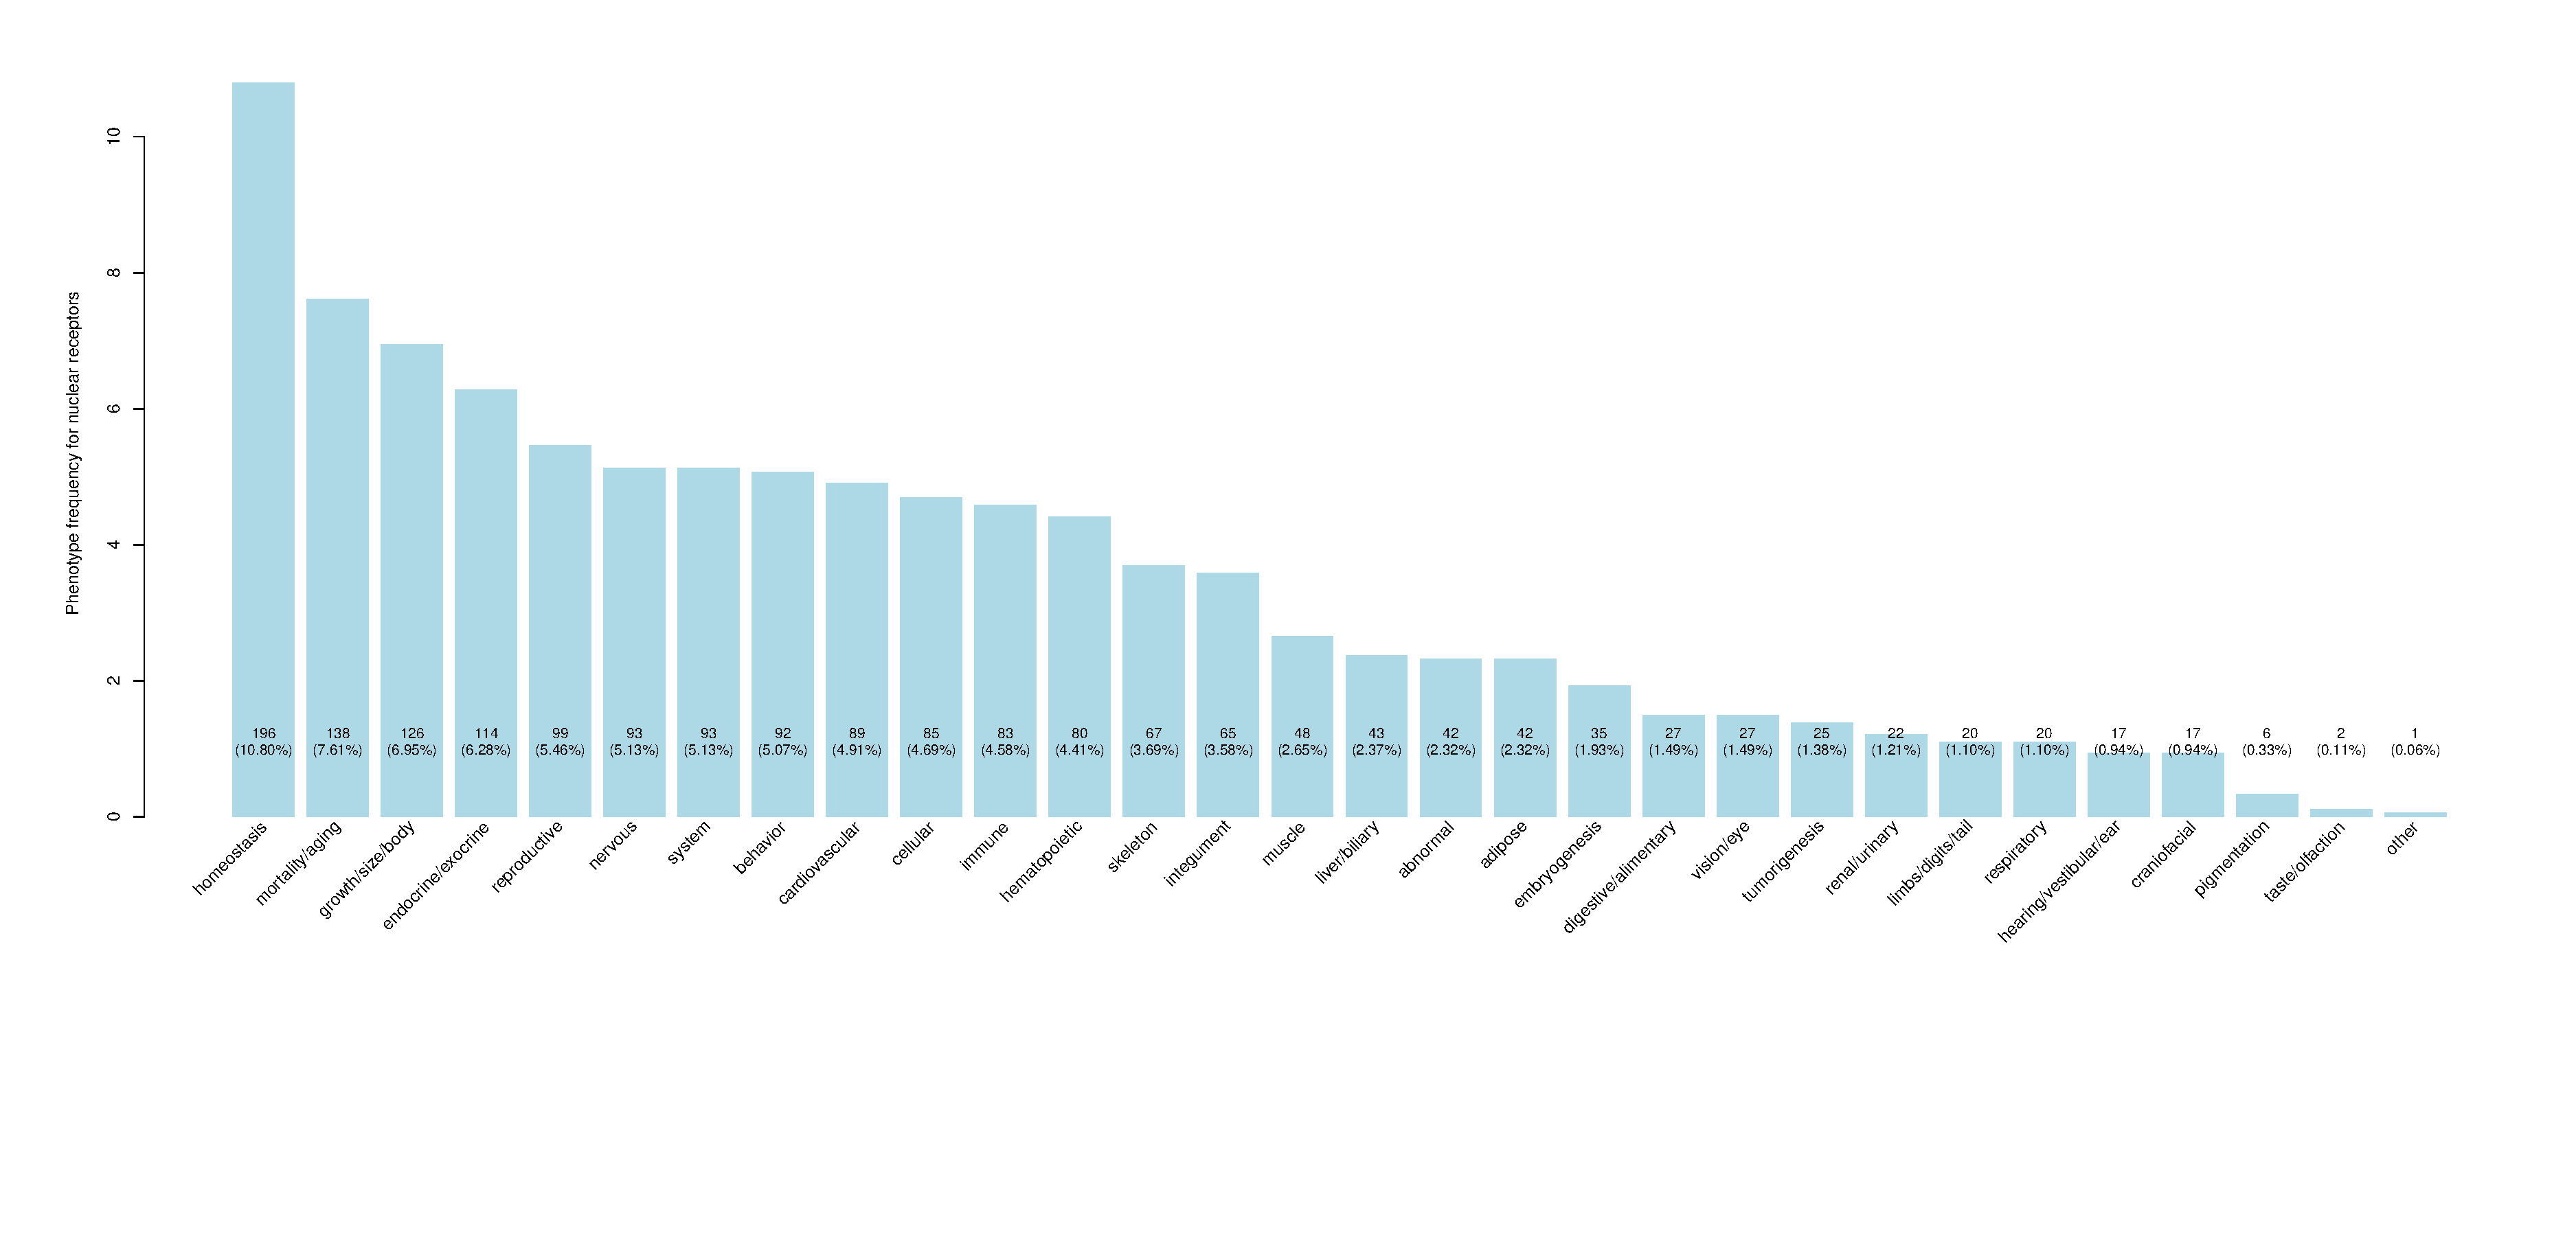
\includegraphics[width=\linewidth]{pics/mgi_phenotypes_distribution.pdf}
	\captionsetup{margin=12pt,format=plain,font=footnotesize,labelfont=bf}
 	\caption{\footnotesize{\textbf{MGI phenotypes}. 
	~~~~~~~\\
	Mouse Genome Informatics phenotype distribution over the nuclear receptors.}}
	\label{fig:mgi_pheotypes_distribution}
\end{figure}
~~~~~~~\\

%Figure~\ref{fig:mgi_pheotypes_distribution} bla bla 
\begin{figure}[H]
	\centering
	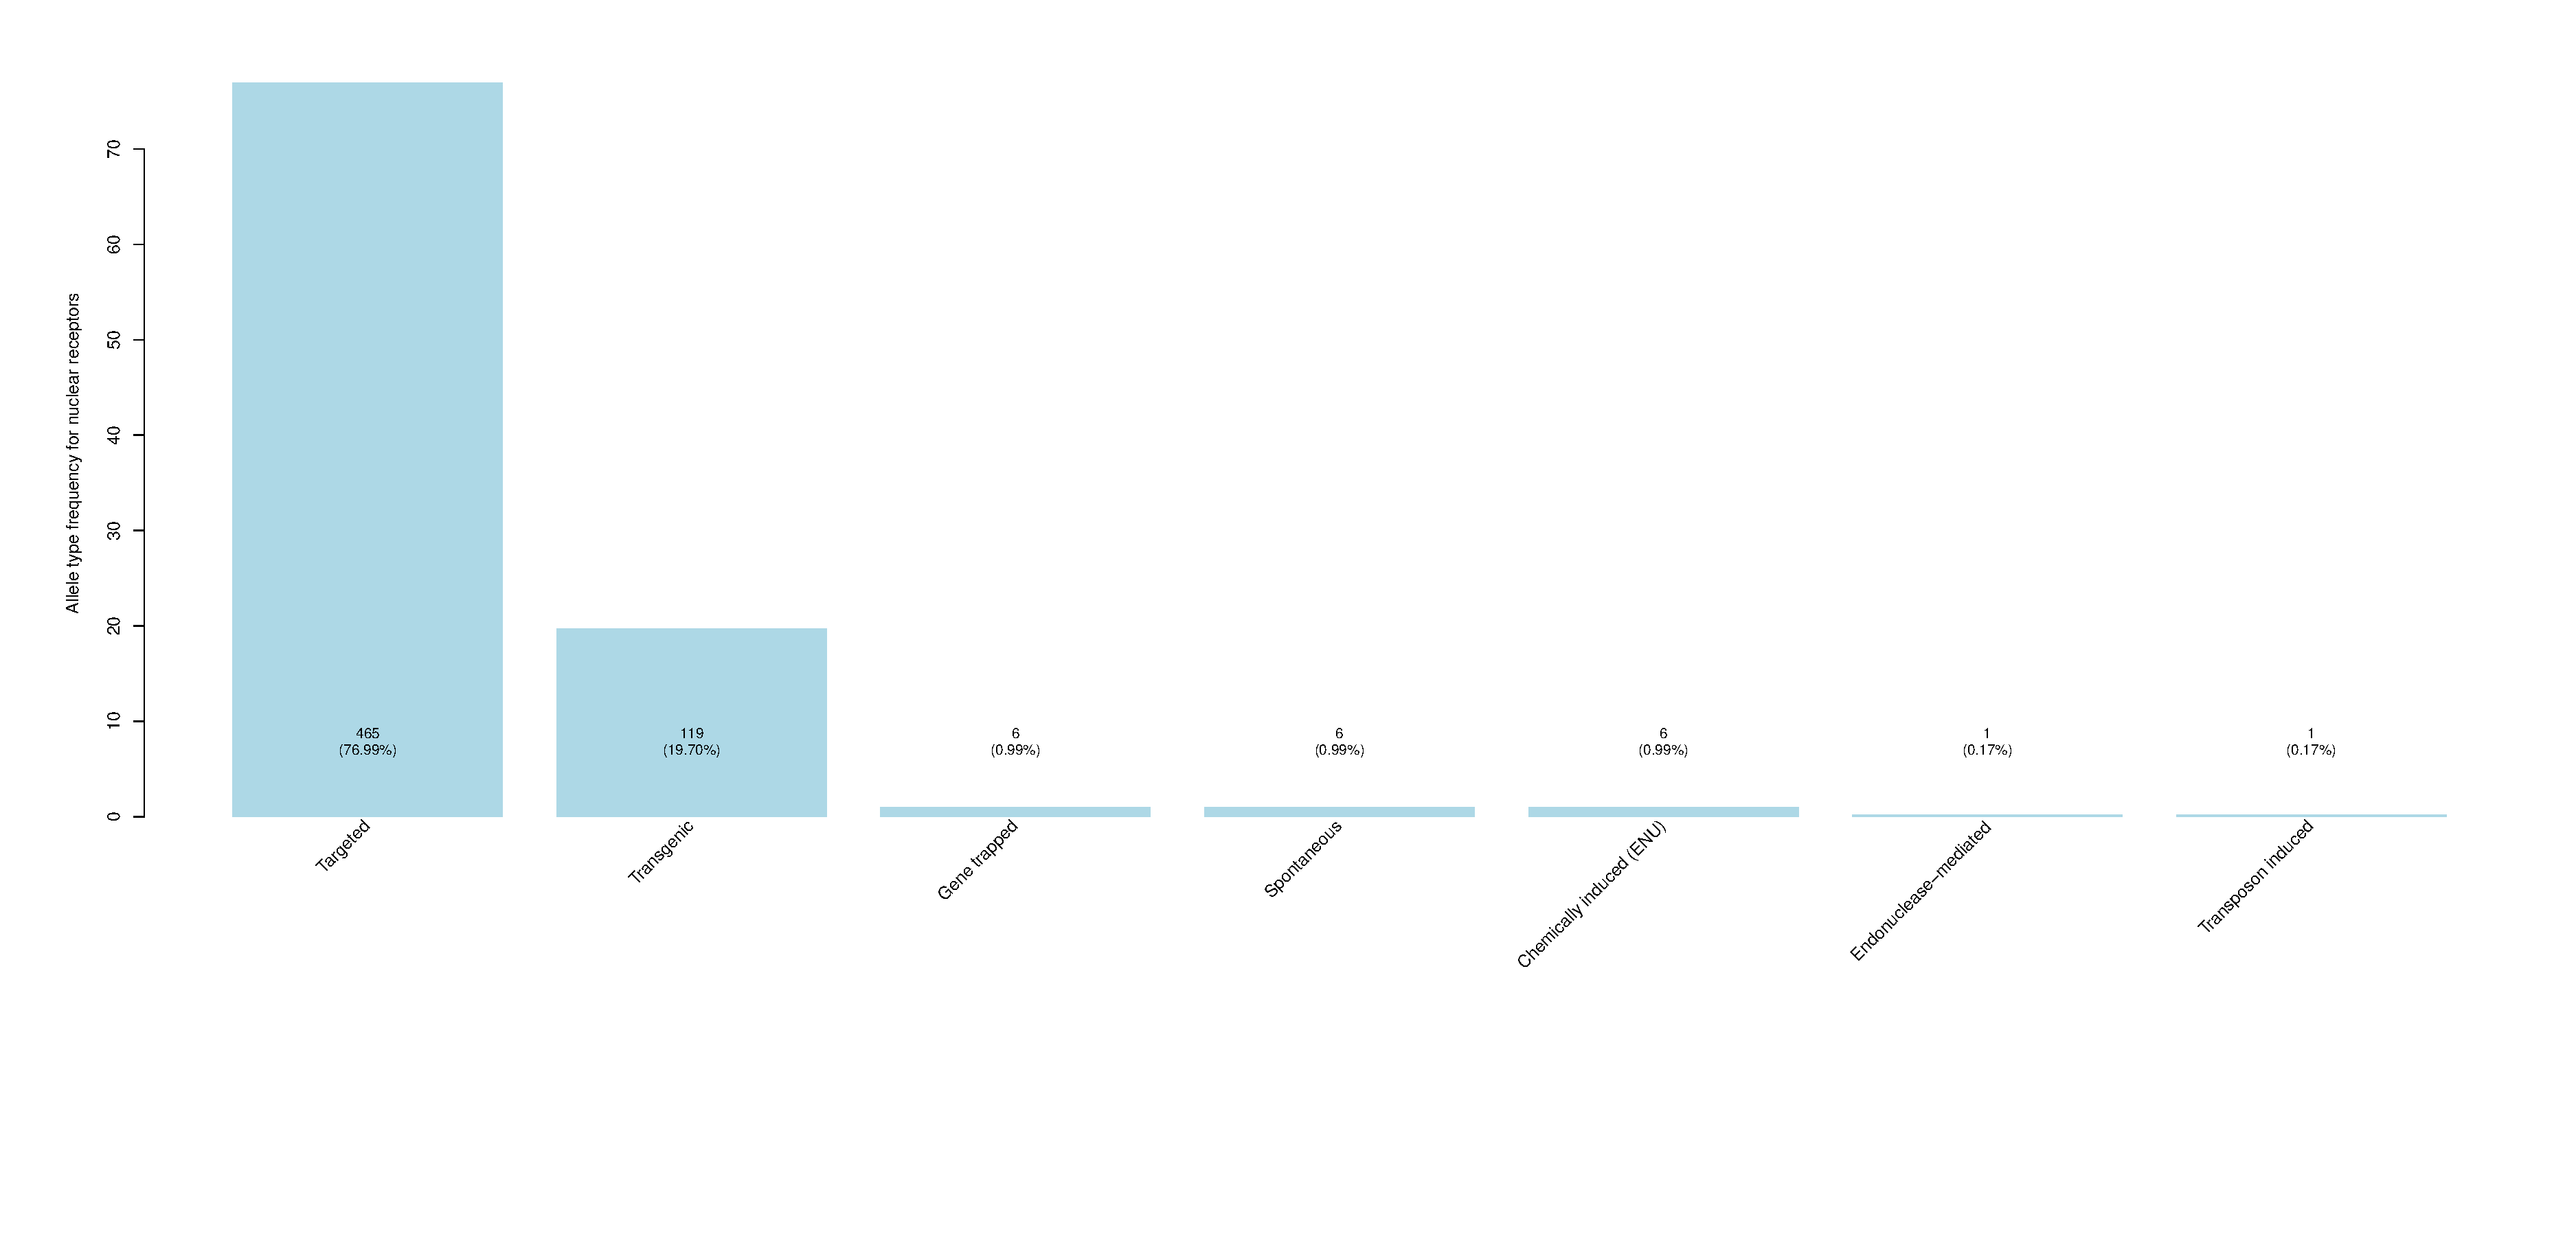
\includegraphics[width=\linewidth]{pics/mgi_types_distribution.pdf}
	\captionsetup{margin=12pt,format=plain,font=footnotesize,labelfont=bf}
 	\caption{\footnotesize{\textbf{MGI allele types}. 
	~~~~~~~\\
	Mouse Genome Informatics allele type distribution over the nuclear receptors.}}
	\label{fig:mgi_types_distribution}
\end{figure}
~~~~~~~\\

\begin{figure}[H]
	\centering
	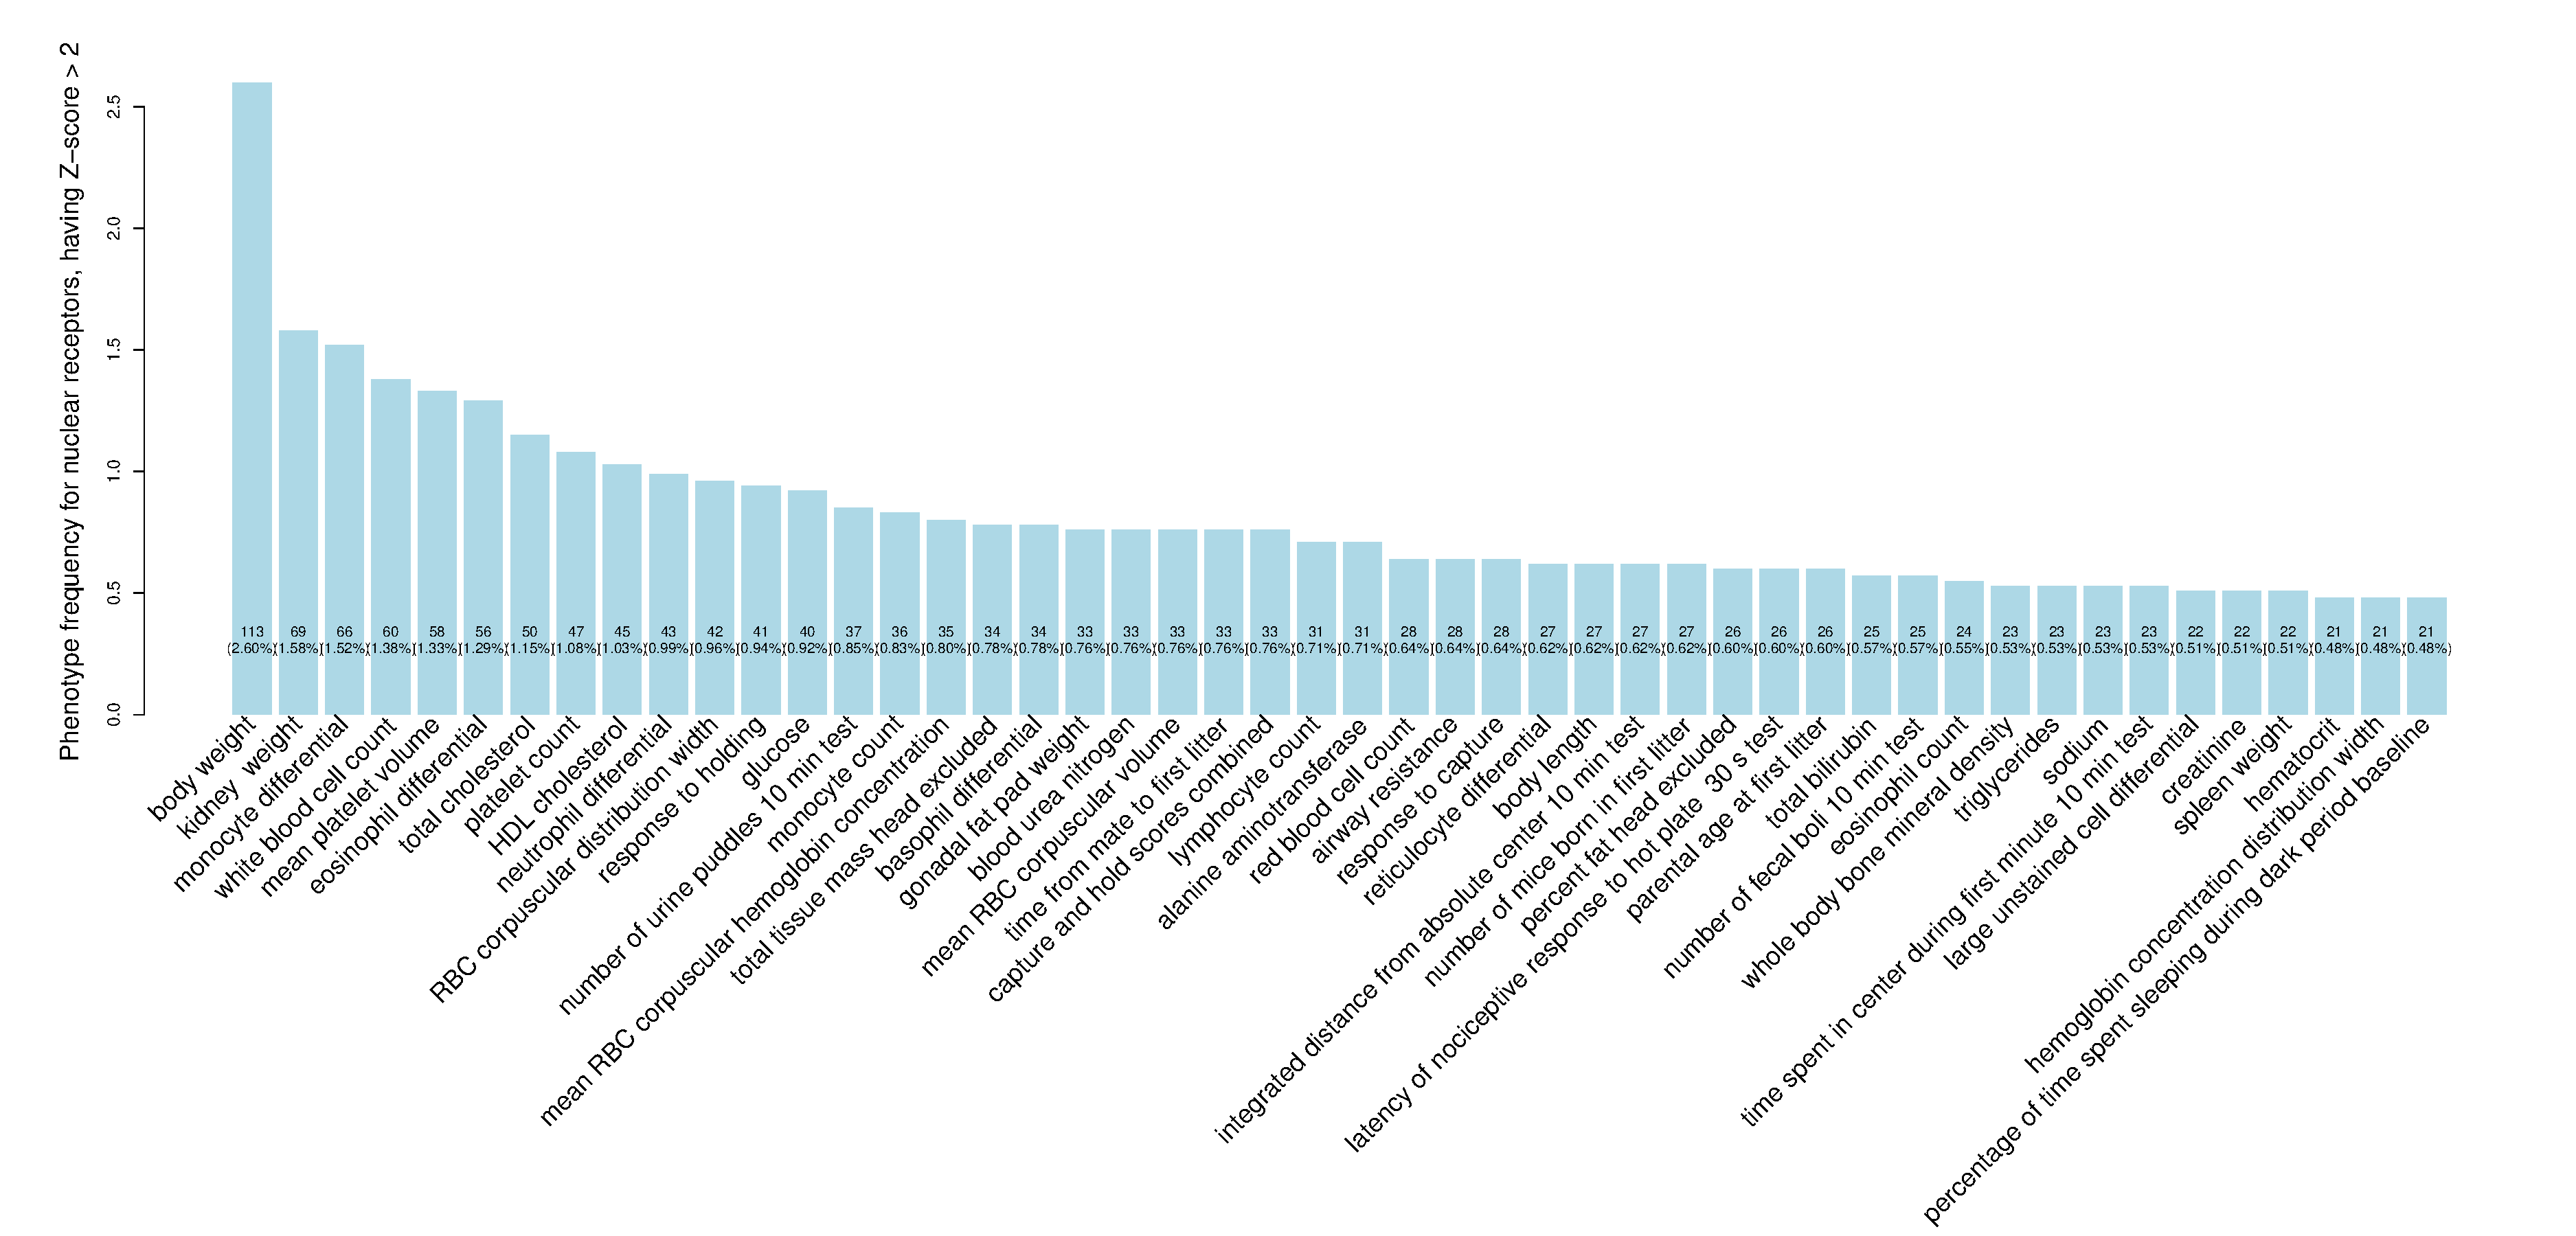
\includegraphics[width=\linewidth]{pics/mpi_phenotypes_distribution_zscore2.pdf}
	\captionsetup{margin=12pt,format=plain,font=footnotesize,labelfont=bf}
 	\caption{\footnotesize{\textbf{MPD phenotypes, having Z-score $>$ 2}. 
	~~~~~~~\\
	Mouse Phenotype Database phenotype distribution over the nuclear receptors, having Z-score $>$ 2}}
	\label{fig:mpi_pheotypes_distribution_zscore2}
\end{figure}
~~~~~~~\\

\begin{figure}[H]
	\centering
	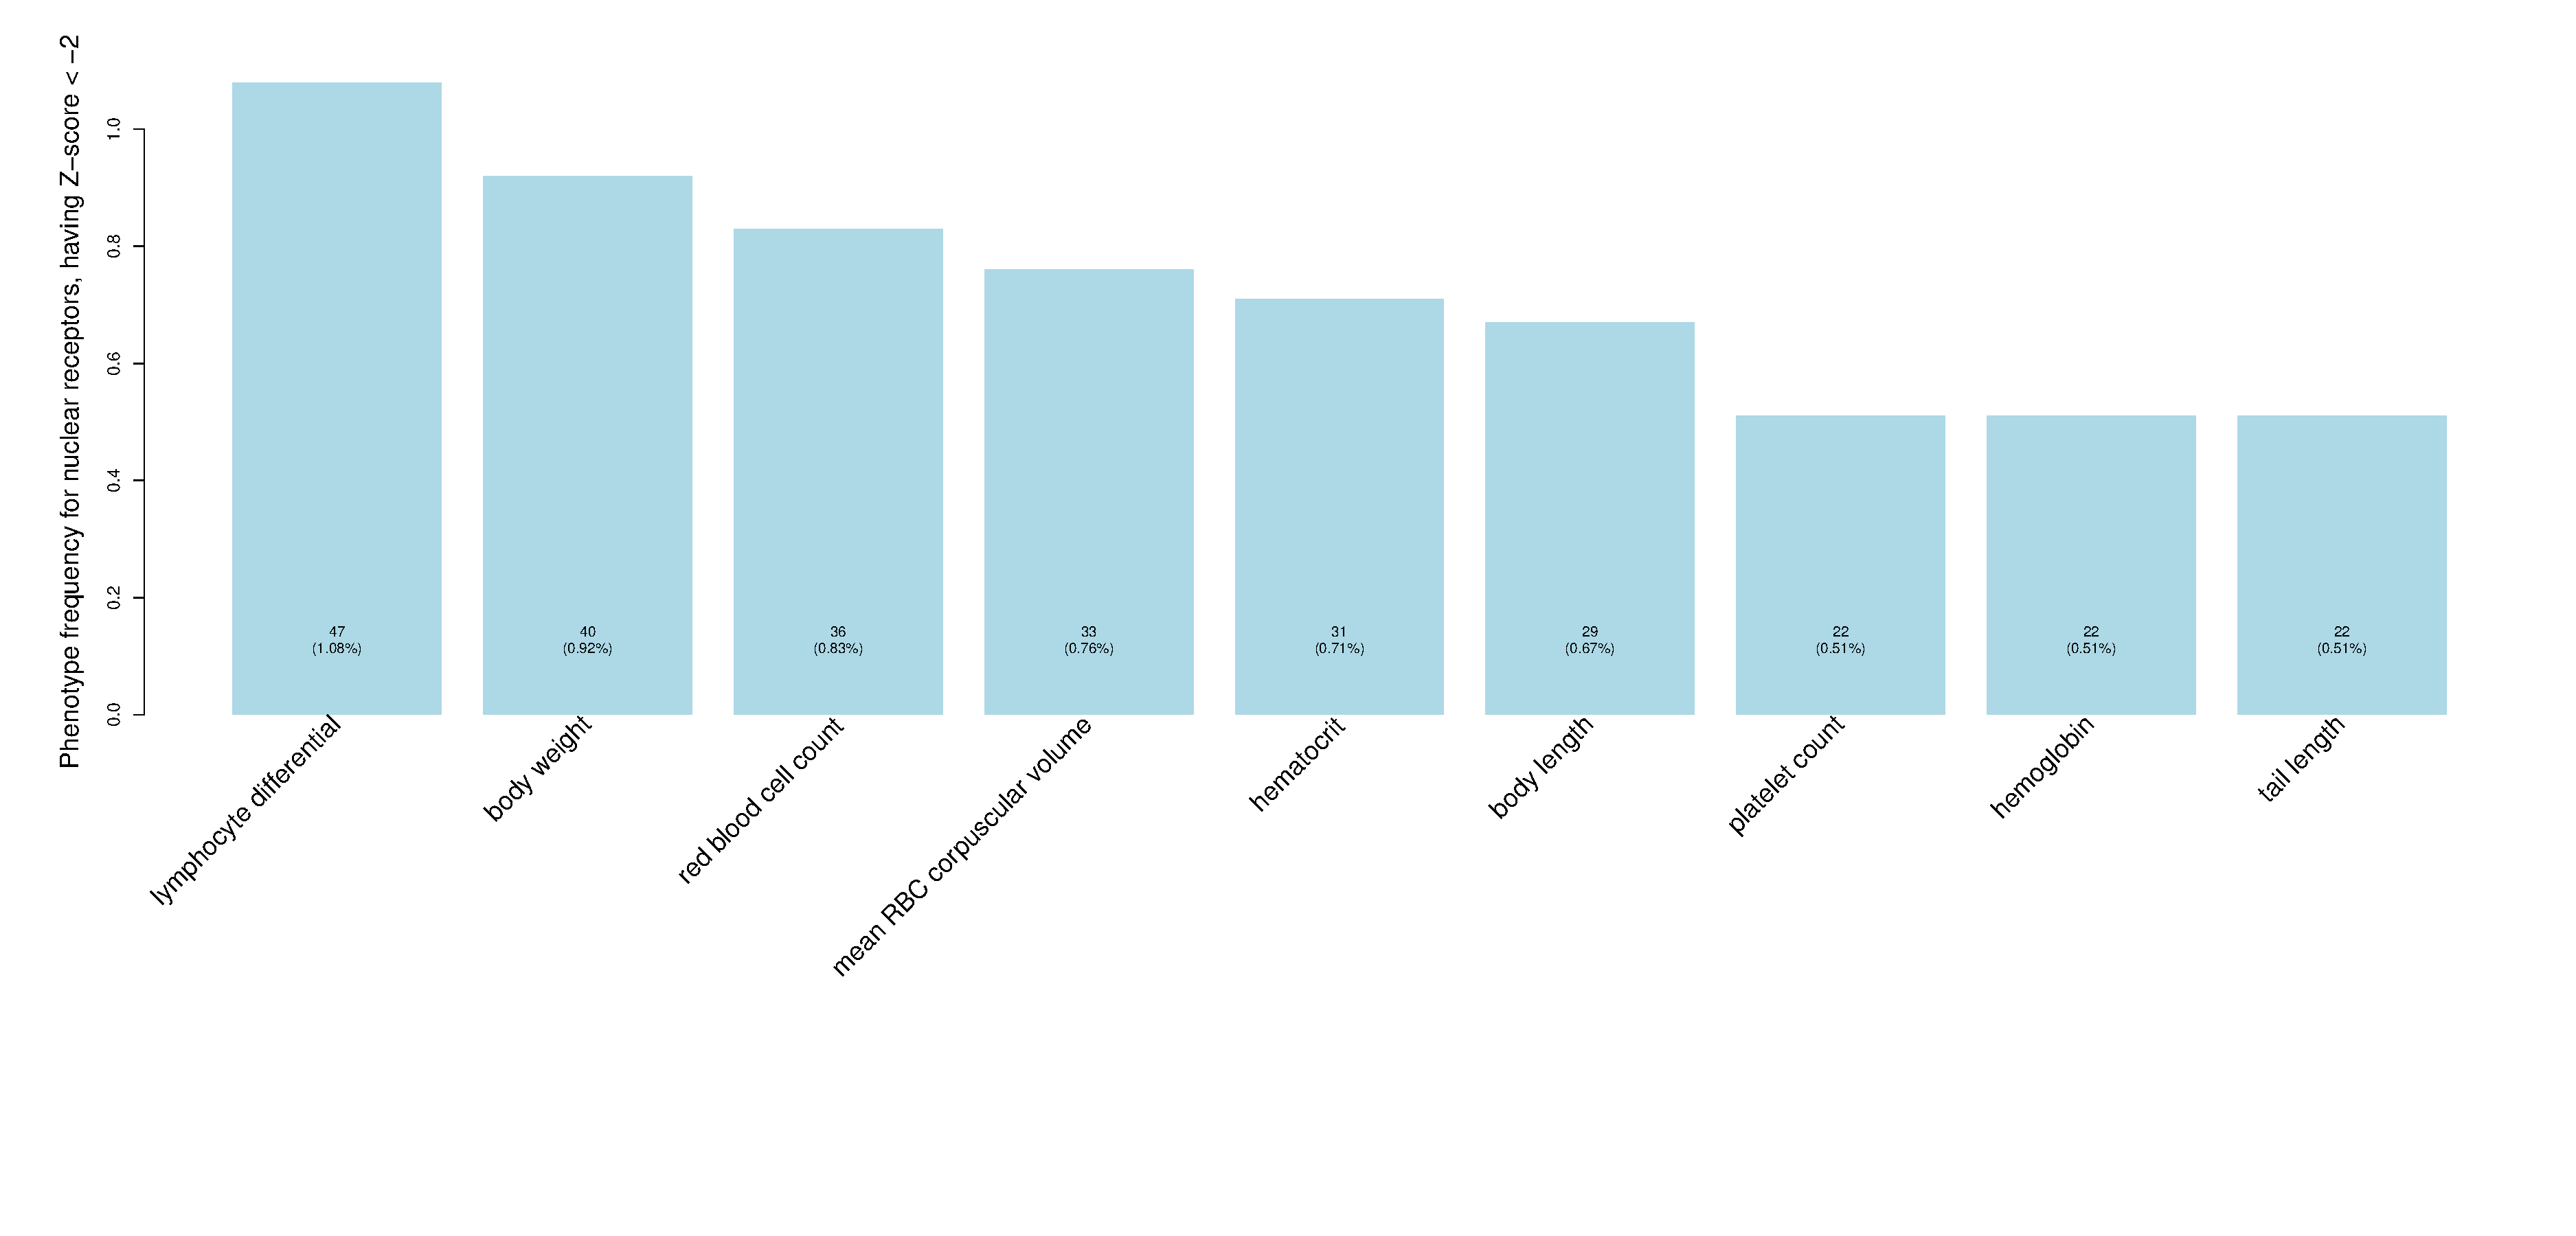
\includegraphics[width=\linewidth]{pics/mpi_phenotypes_distribution_zscore2_neg.pdf}
	\captionsetup{margin=12pt,format=plain,font=footnotesize,labelfont=bf}
 	\caption{\footnotesize{\textbf{MPD phenotypes, having Z-score $<$ -2}. 
	~~~~~~~\\
	Mouse Phenotype Database phenotype distribution over the nuclear receptors, having Z-score $<$ -2}}
	\label{fig:mpi_pheotypes_distribution_zscore2_neg}
\end{figure}
~~~~~~~\\

\begin{figure}[H]
	\centering
	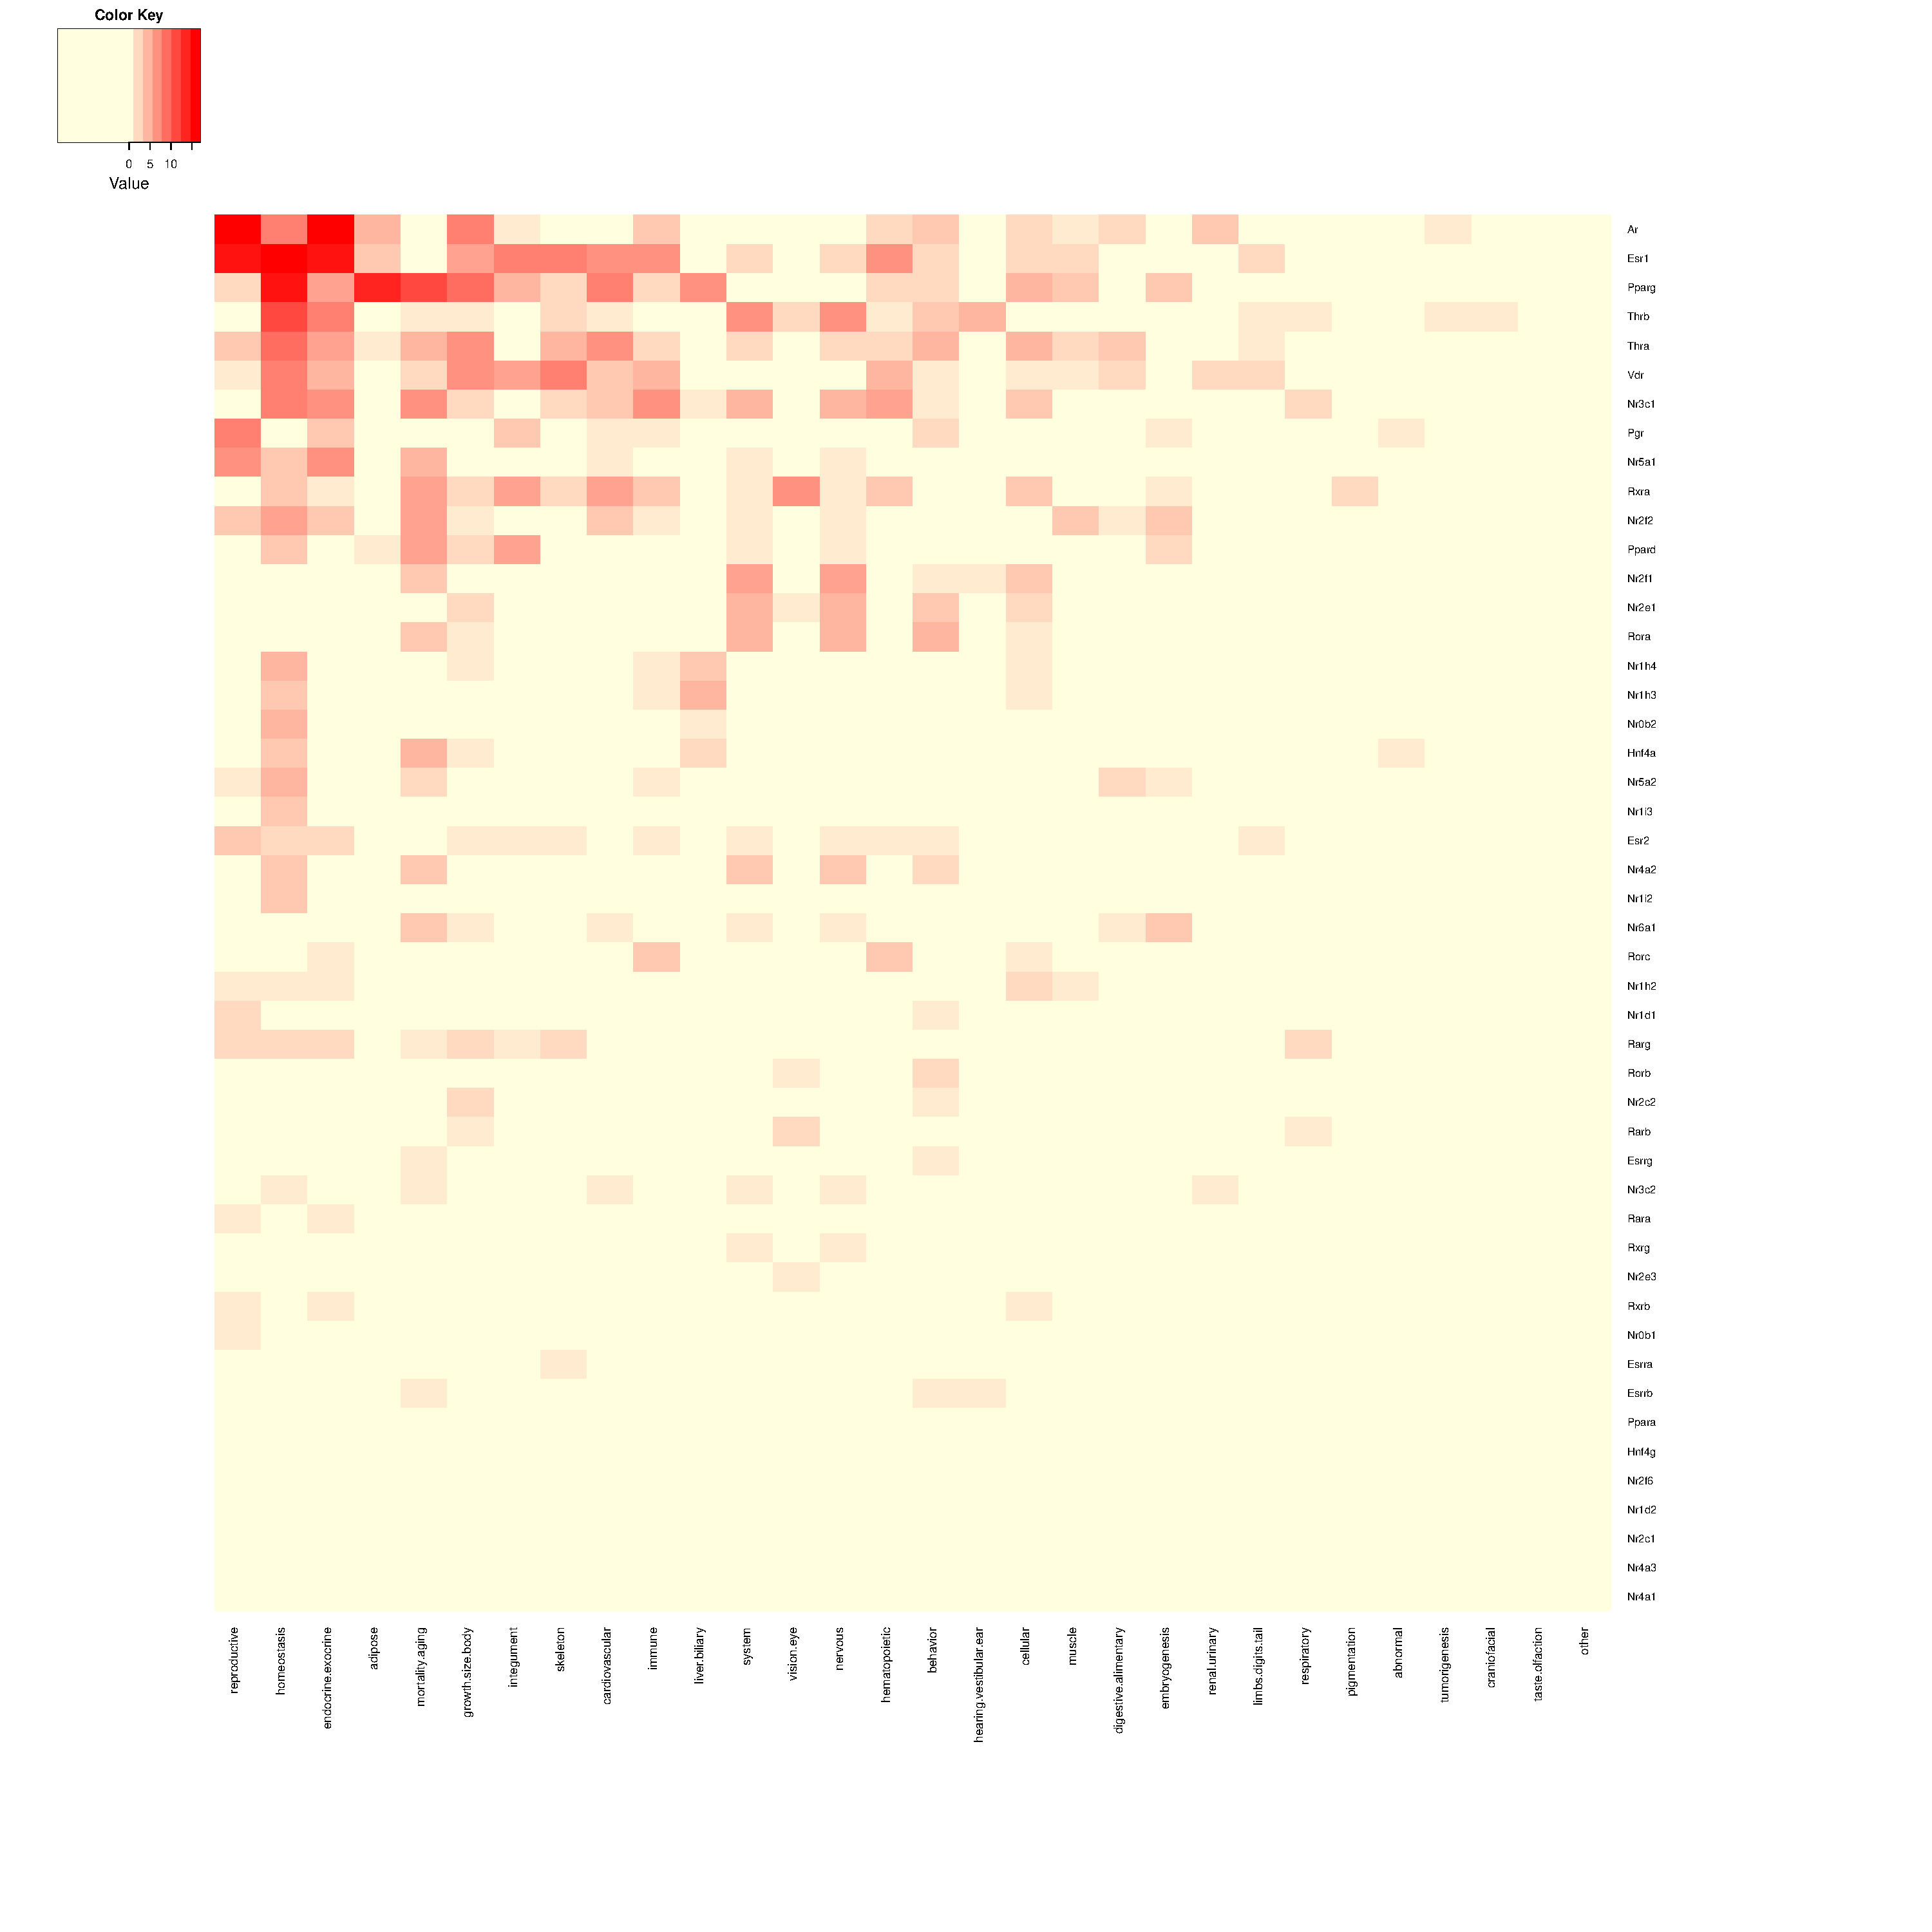
\includegraphics[width=\linewidth]{pics/mgi_phenotypes_nr.pdf}
	\captionsetup{margin=12pt,format=plain,font=footnotesize,labelfont=bf}
 	\caption{\footnotesize{\textbf{MGI phenotype - nuclear receptor associations}. 
	~~~~~~~\\
	Mouse Genome Informatics phenotype occurrence frequency among the nuclear receptors.}}
	\label{fig:mgi_pheotypes_nr}
\end{figure}
~~~~~~~\\

\begin{figure}[H]
	\centering
	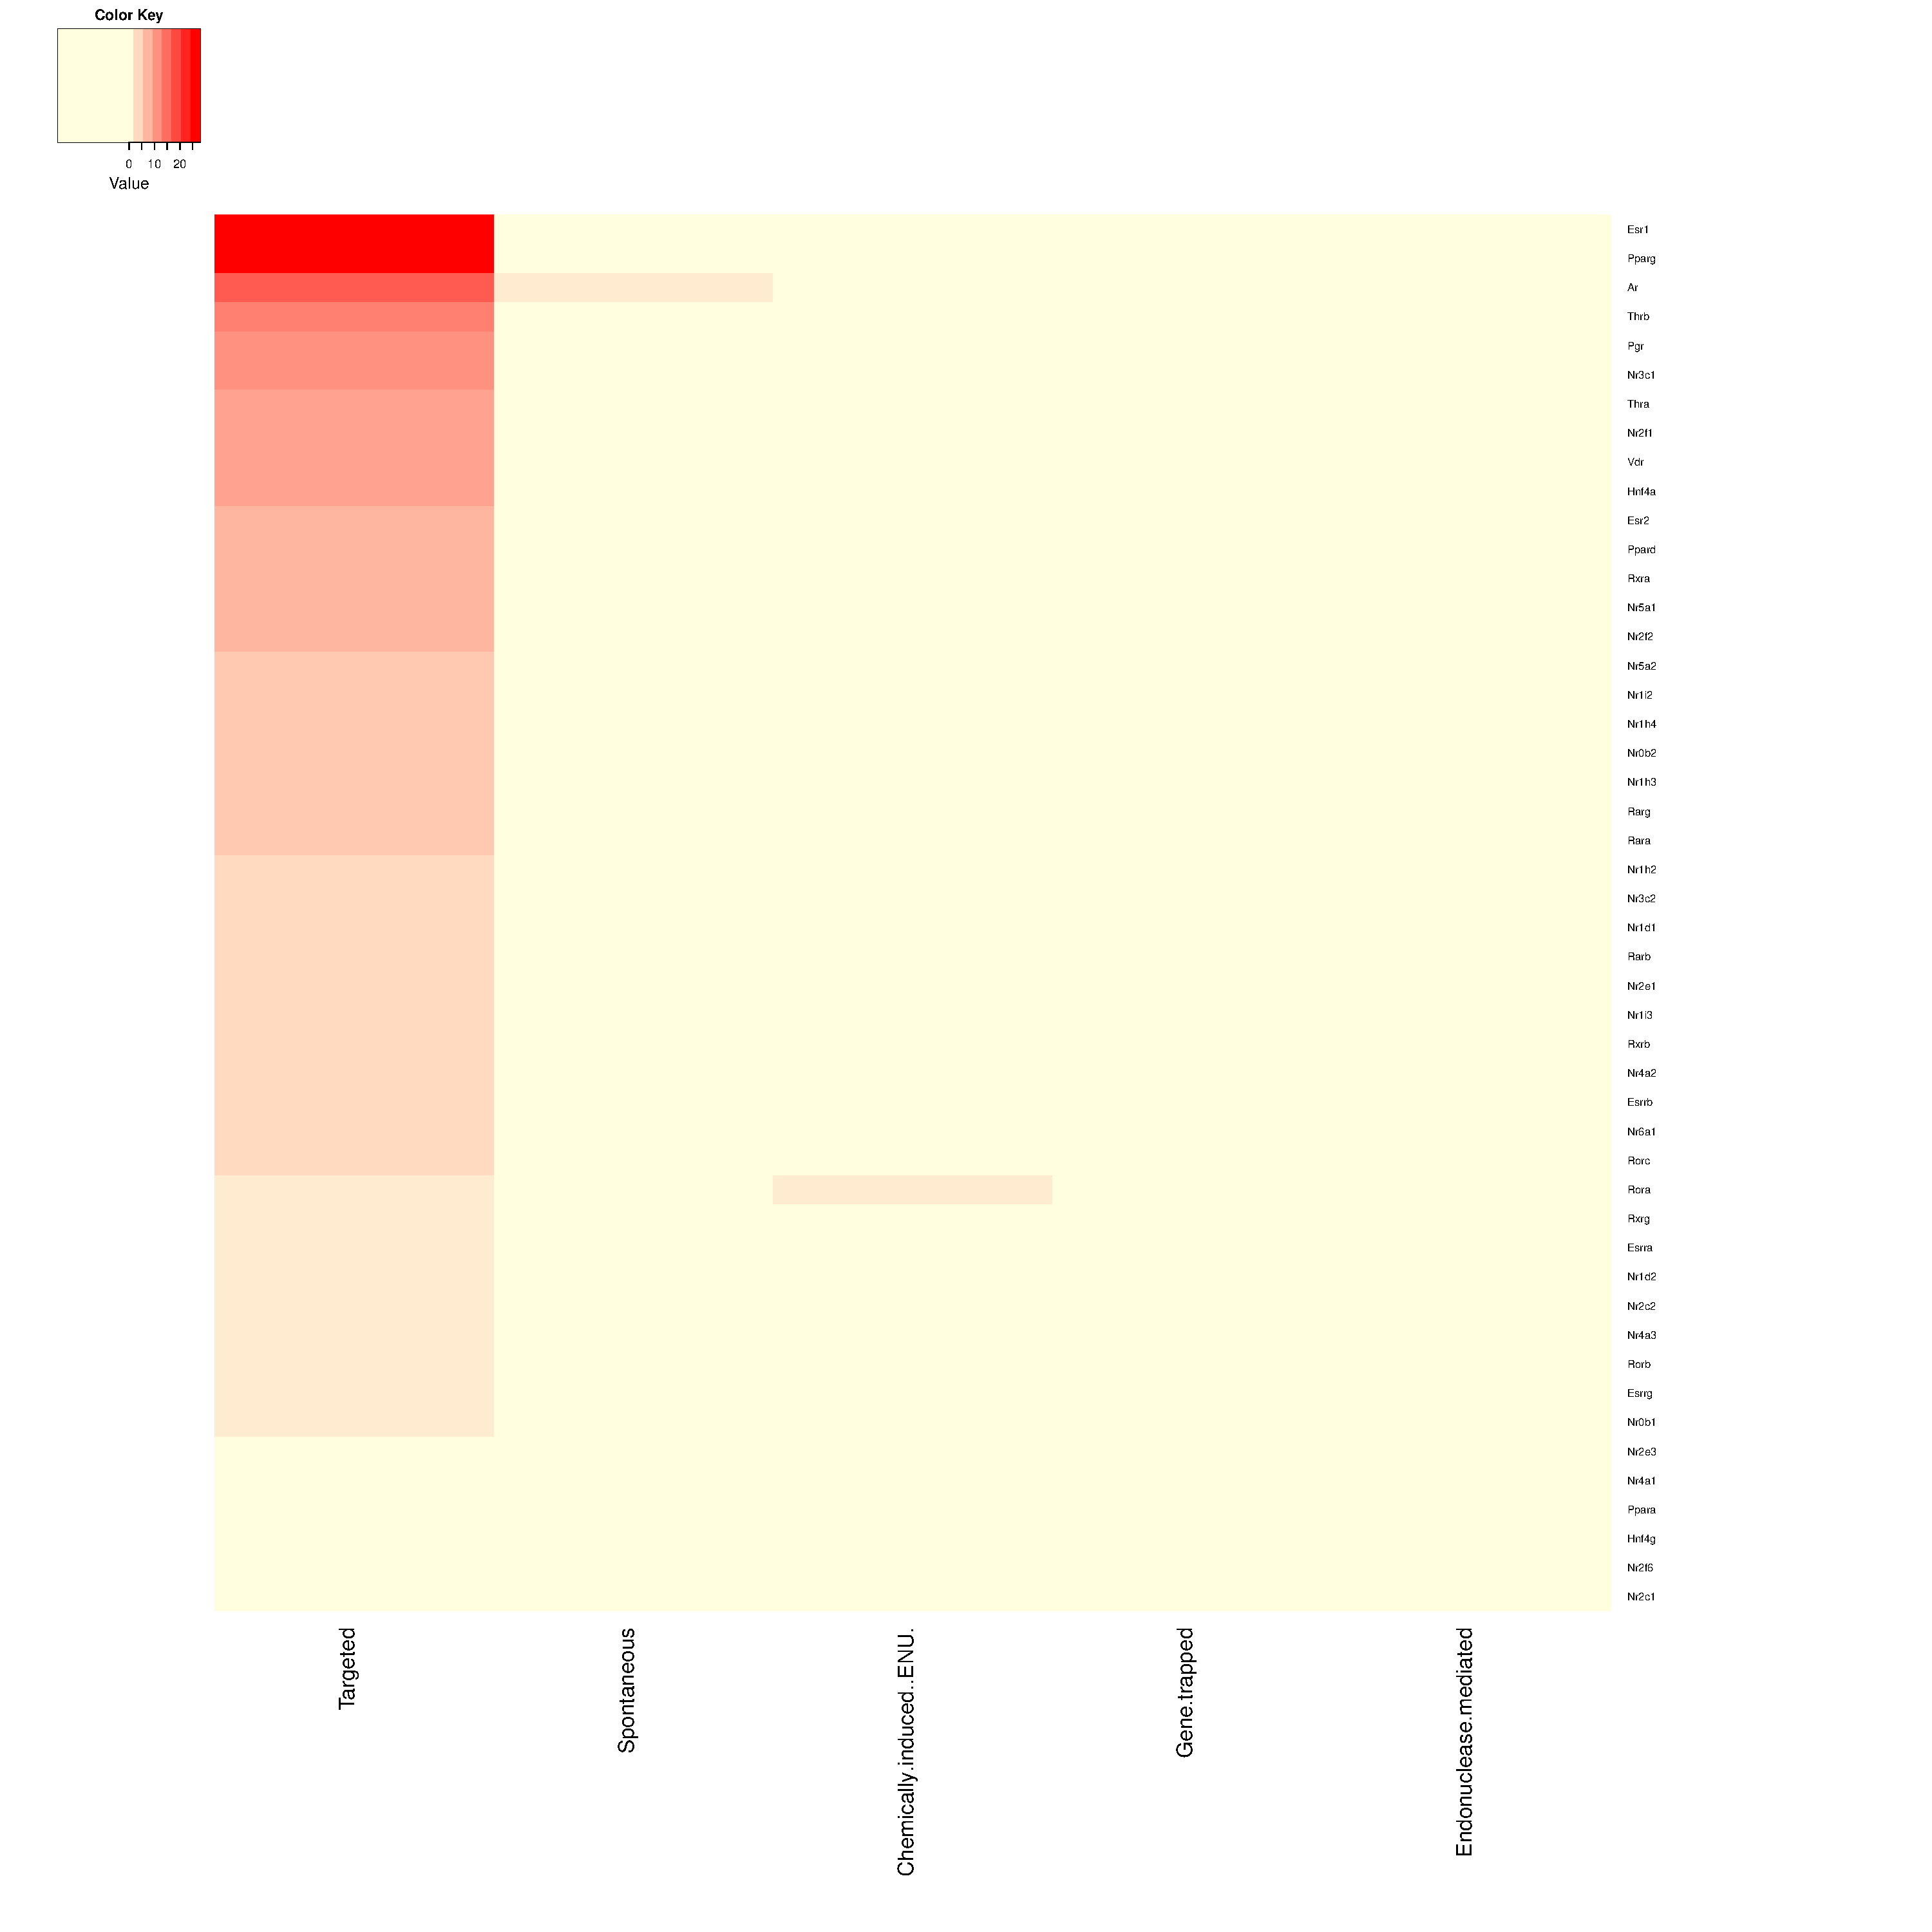
\includegraphics[width=\linewidth]{pics/mgi_types_nr.pdf}
	\captionsetup{margin=12pt,format=plain,font=footnotesize,labelfont=bf}
 	\caption{\footnotesize{\textbf{MGI allele type - nuclear receptor associations}. 
	~~~~~~~\\
	Mouse Genome Informatics allele type occurrence frequency among the nuclear receptors.}}
	\label{fig:mgi_types_nr}
\end{figure}
~~~~~~~\\

\begin{figure}[H]
	\centering
	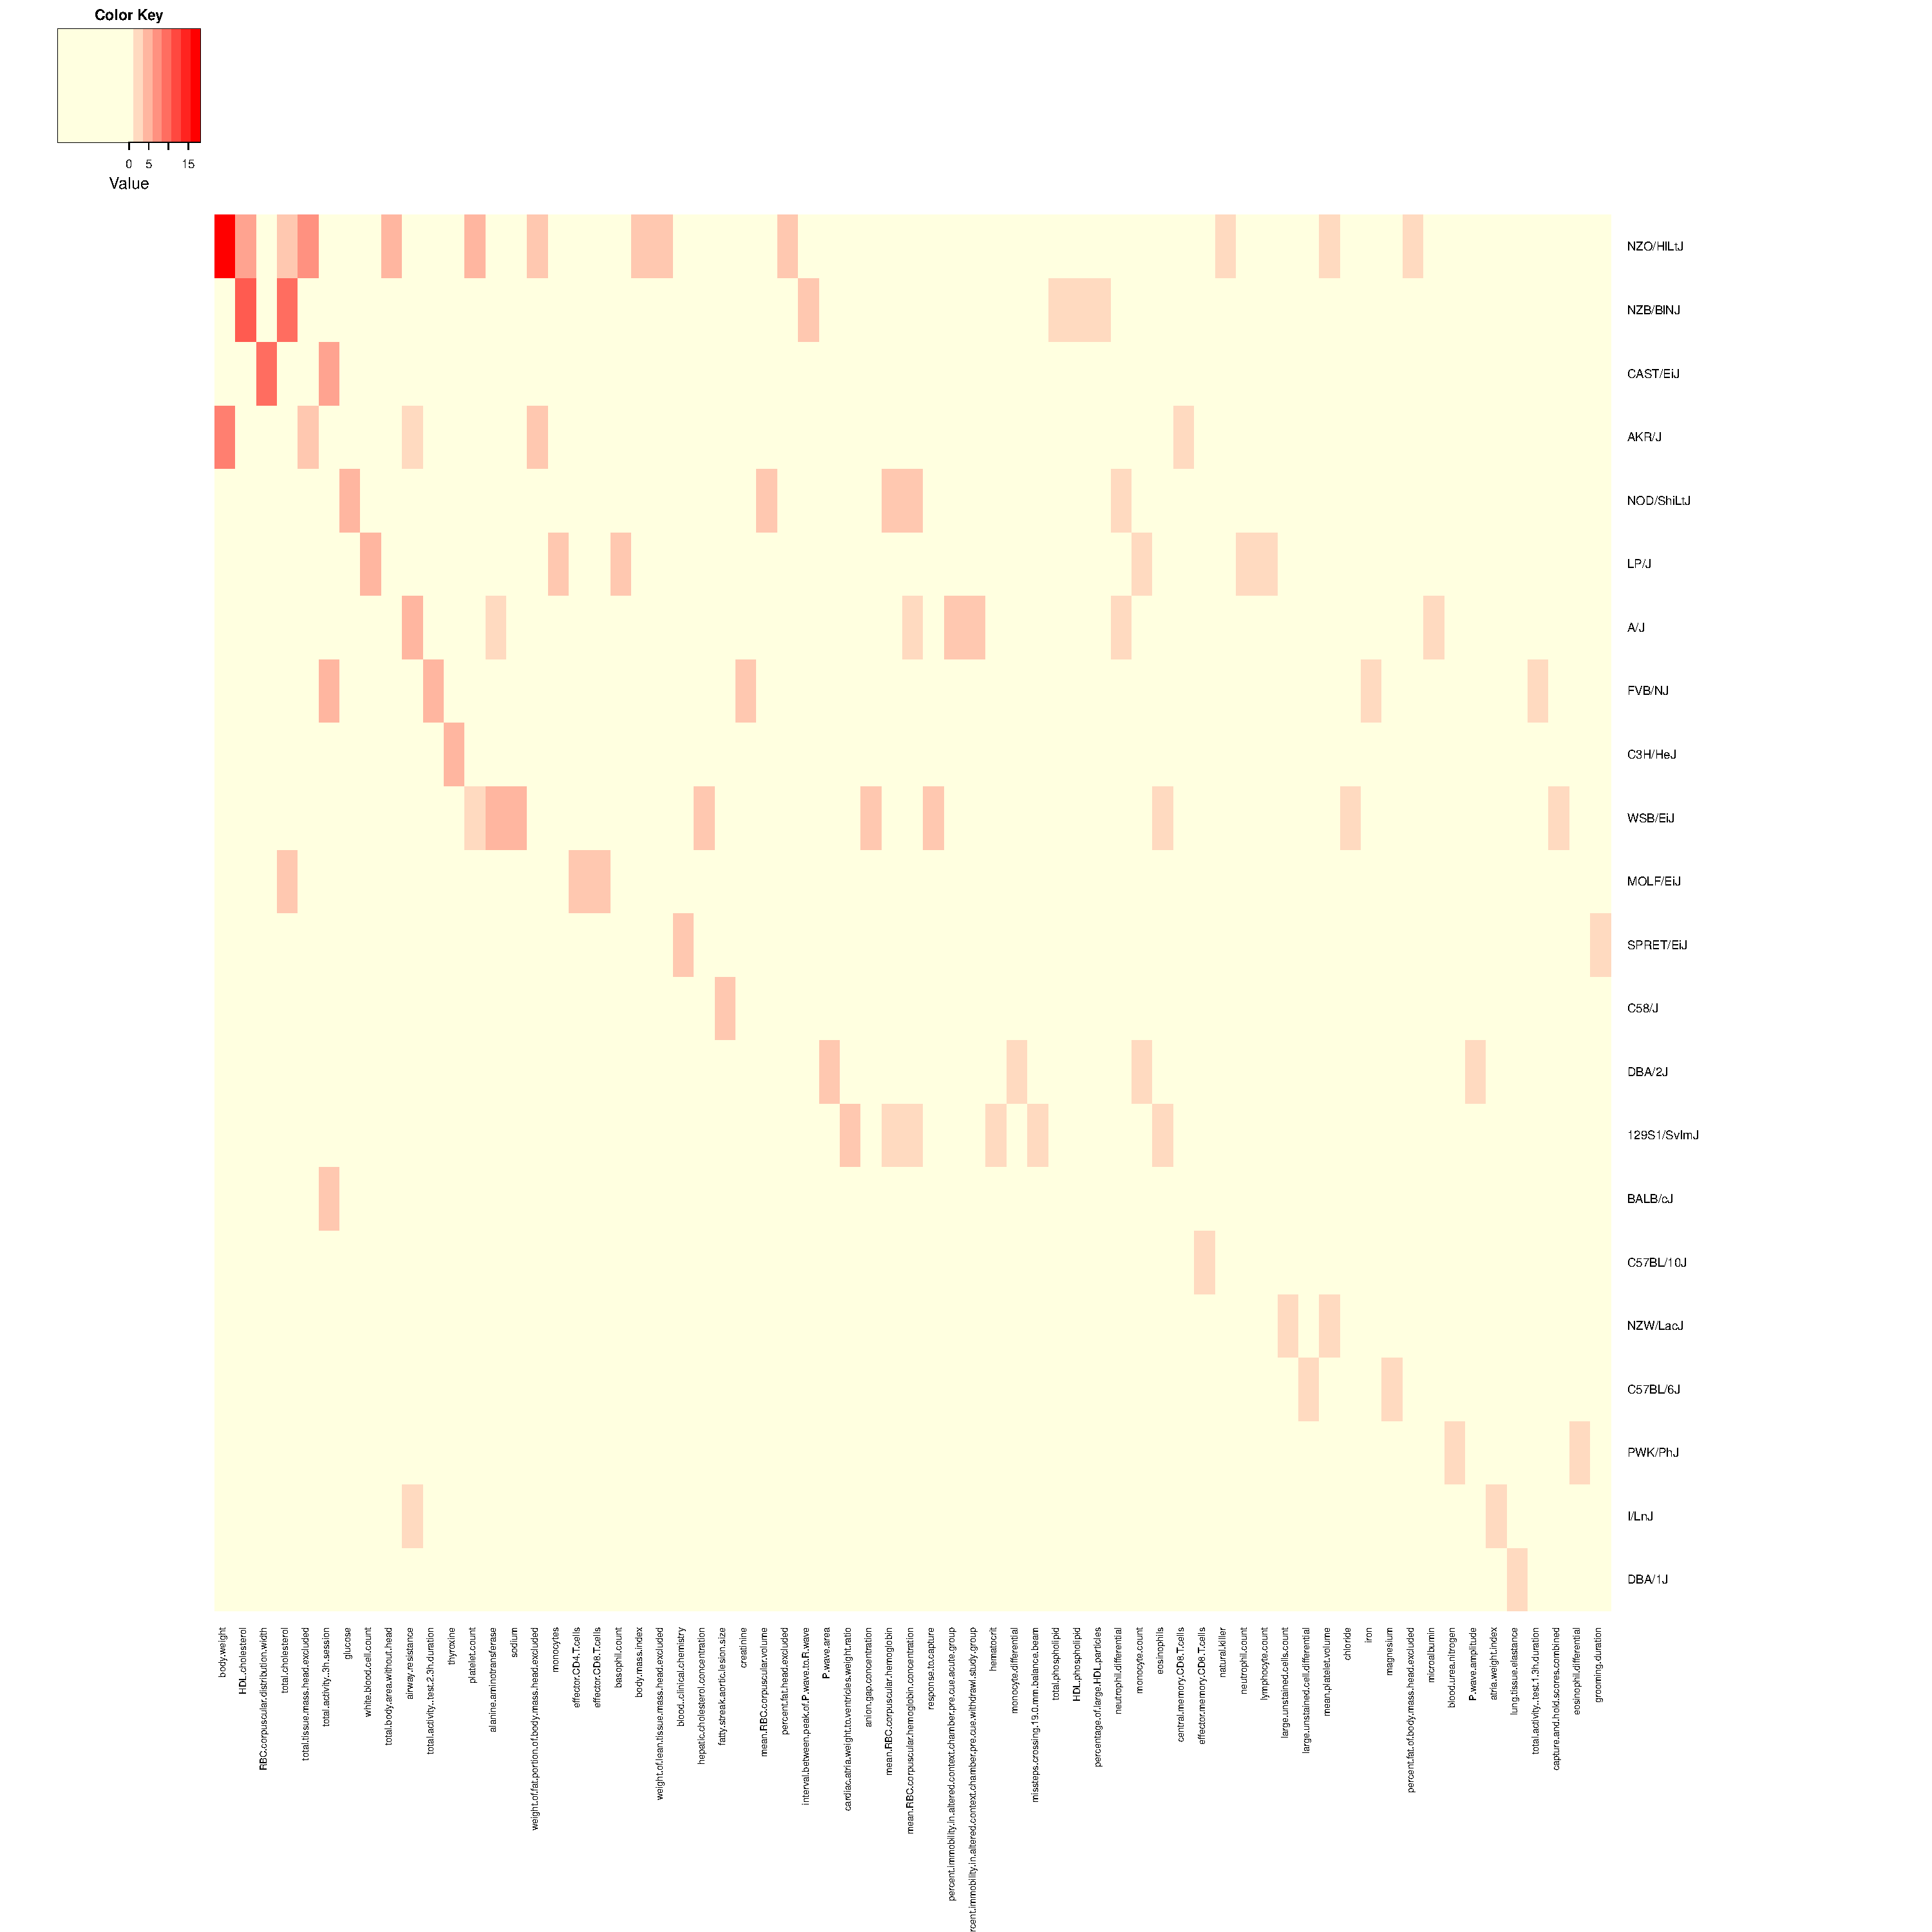
\includegraphics[width=\linewidth]{pics/mpi_phenotypes_strain_zscore2.pdf}
	\captionsetup{margin=12pt,format=plain,font=footnotesize,labelfont=bf}
 	\caption{\footnotesize{\textbf{MPD phenotype - strain associations, having Z-score $>$ 2}. 
	~~~~~~~\\
	Mouse Phenome Database phenotype occurrence frequency among the strains associated with the nuclear receptors, having Z-score $>$ 2}}
	\label{fig:mgi_pheotypes_strain_zscore2}
\end{figure}
~~~~~~~\\

\begin{figure}[H]
	\centering
	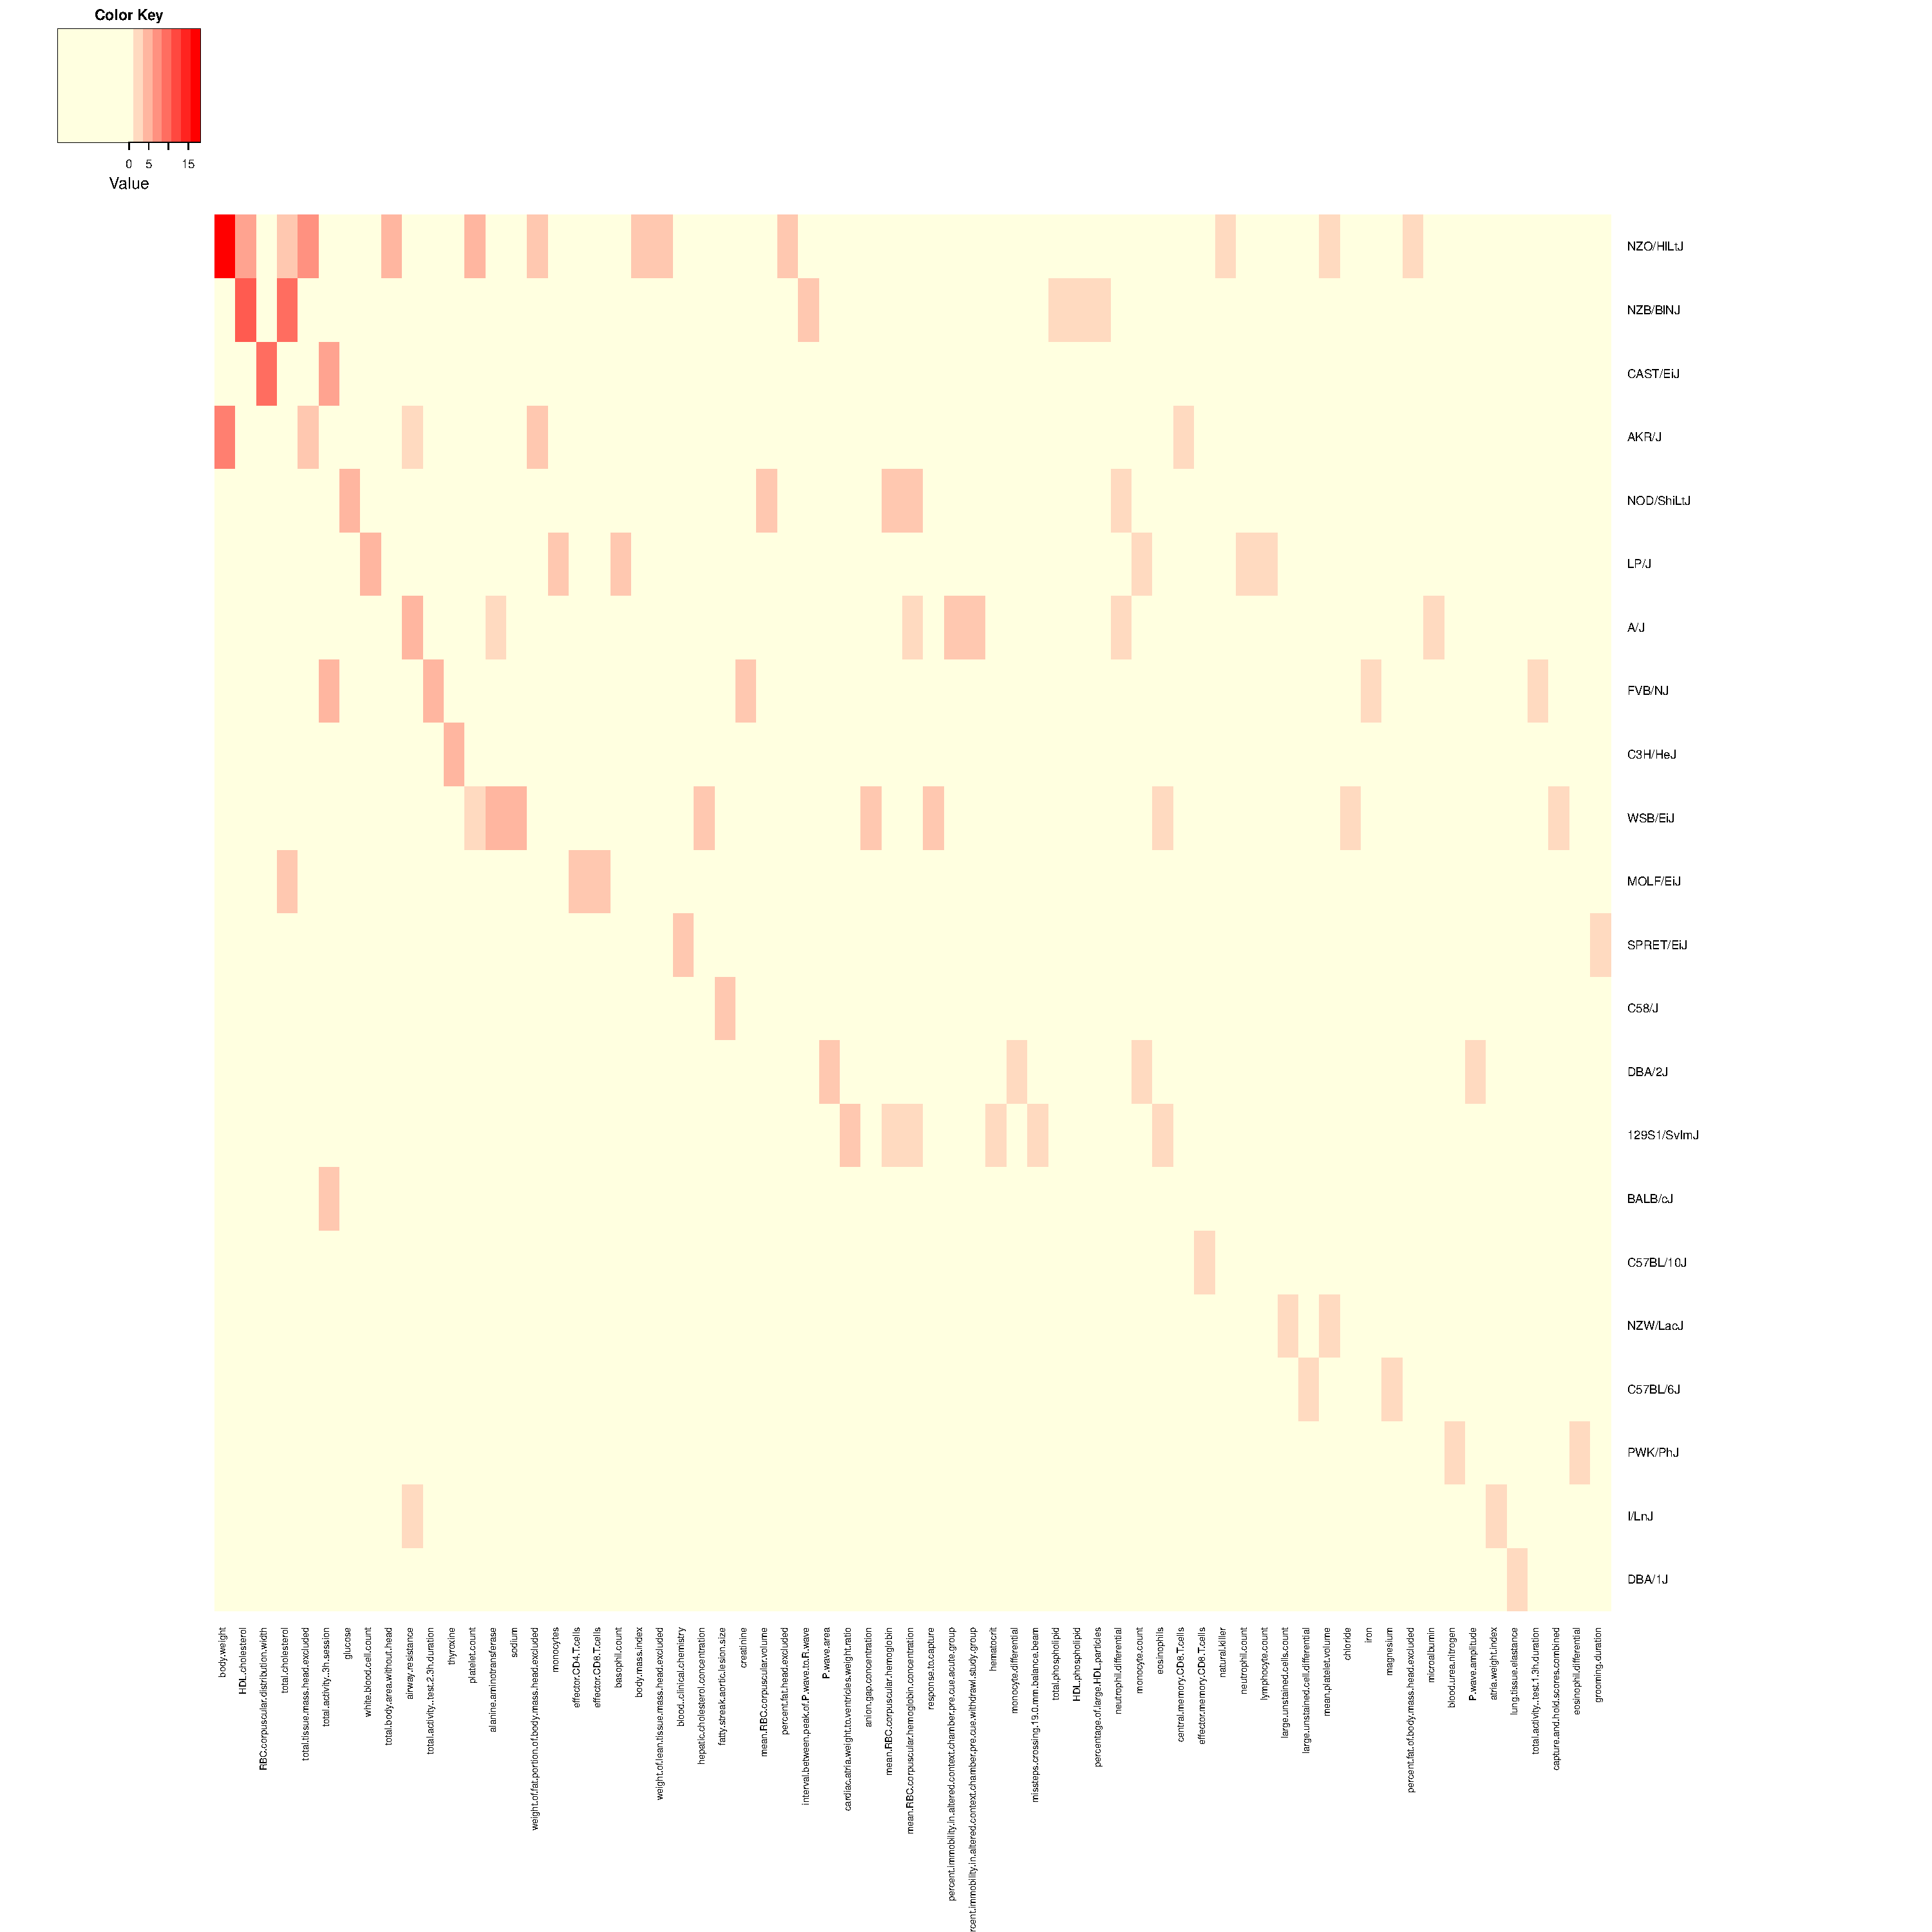
\includegraphics[width=\linewidth]{pics/mpi_phenotypes_strain_zscore2.pdf}
	\captionsetup{margin=12pt,format=plain,font=footnotesize,labelfont=bf}
 	\caption{\footnotesize{\textbf{MPD phenotype - strain associations, having Z-score $<$ -2}. 
	~~~~~~~\\
	Mouse Phenome Database phenotype occurrence frequency among the strains associated with the nuclear receptors, having Z-score $<$ -2}}
	\label{fig:mgi_pheotypes_strain_zscore2_neg}
\end{figure}

%------------------------------------------------
\section{Discussion and Outlook}

Blabla 

%------------------------------------------------
\section{Acknowledgments} % The \section*{} command stops section numbering

Our gratitude to Prof. Dr. H. W. Mewes for offering us the topic and the opportunity to work with the Helmholz Zentrum research centre in Munich. Many thanks to our supervisor, Dr. Desislava Boyanova for all the input and ideas, discussions, advices and foremost her useful and critical suggestions which motivated us a lot. Last but not least, we would like to thank our fellow colleagues for their support, as well as the entire \emph{Helmholz Zentrum} group. 
%----------------------------------------------------------------------------------------
%	REFERENCE LIST
%----------------------------------------------------------------------------------------
\phantomsection
\bibliographystyle{unsrt}
\bibliography{sample}

%----------------------------------------------------------------------------------------

\end{document}